\textbf{Pour les exercices \ref{AireBasique1} à \ref{AireBasique12} }: Calculer l'aire de la figure.

\begin{minipage}[t]{0.30\textwidth}
    \exo{Calculer}{AireBasique1}\\
    \begin{figure}[H]
        \centering
        \begin{tikzpicture}
            \draw (0,0)--node[midway,above] {4} (3,0)--node[midway,left] {2} (3,2)--(0,2)--cycle;
        \end{tikzpicture}
    \end{figure}
\end{minipage}
\hfill
\begin{minipage}[t]{0.30\textwidth}
    \exo{Calculer}{AireBasique2}\\
    \begin{figure}[H]
        \centering
        \begin{tikzpicture}
            \draw (0,0)--node[midway,above] {3} (2,0)--(2,2)--(0,2)--cycle;
        \end{tikzpicture}
    \end{figure}
\end{minipage}
\hfill
\begin{minipage}[t]{0.30\textwidth}
    \exo{Calculer}{AireBasique3}\\
    \begin{figure}[H]
        \centering
        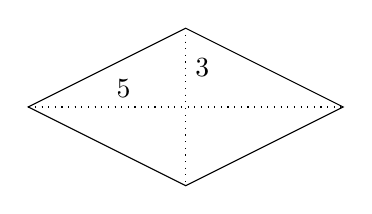
\begin{tikzpicture}
            \draw (0,0)-- (2,1)-- (4,0)--(2,-1)--cycle;
            \draw[dotted] (2,1)-- (2,0) node [midway,right] {3};
            \draw[dotted] (2,1)-- (2,-1) ;
            \draw[dotted] (0,0)-- (2,0) node [midway, above right] {5};
            \draw[dotted] (0,0)-- (4,0) ;
        \end{tikzpicture}
    \end{figure}
\end{minipage}

\begin{minipage}[t]{0.30\textwidth}
    \exo{Calculer}{AireBasique4}\\
    \begin{figure}[H]
        \centering
        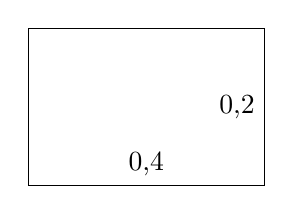
\begin{tikzpicture}
            \draw (0,0)--node[midway,above] {0,4} (3,0)--node[midway,left] {0,2} (3,2)--(0,2)--cycle;
        \end{tikzpicture}
    \end{figure}
\end{minipage}
\hfill
\begin{minipage}[t]{0.30\textwidth}
    \exo{Calculer}{AireBasique5}\\
    \begin{figure}[H]
        \centering
        \begin{tikzpicture}
            \draw (0,0)--node[midway,above] {1,6} (2,0)--(2,2)--(0,2)--cycle;
        \end{tikzpicture}
    \end{figure}
\end{minipage}
\hfill
\begin{minipage}[t]{0.30\textwidth}
    \exo{Calculer}{AireBasique6}\\
    \begin{figure}[H]
        \centering
        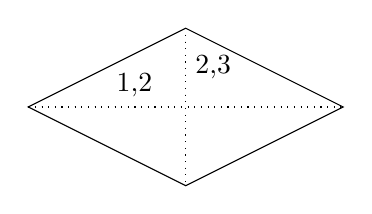
\begin{tikzpicture}
            \draw (0,0)-- (2,1)-- (4,0)--(2,-1)--cycle;
            \draw[dotted] (2,1)-- (2,0) node [midway,right] {2,3};
            \draw[dotted] (2,1)-- (2,-1) ;
            \draw[dotted] (0,0)-- (2,0) node [midway, above right] {1,2};
            \draw[dotted] (0,0)-- (4,0) ;
        \end{tikzpicture}
    \end{figure}
\end{minipage}

\begin{minipage}[t]{0.30\textwidth}
    \exo{Calculer}{AireBasique7}\\
    \begin{figure}[H]
        \centering
        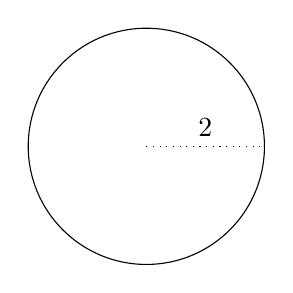
\begin{tikzpicture}
            \draw (0,0) circle (1.5);
            \draw[dotted] (0,0)--(1.5,0) node [midway, above] {2};
        \end{tikzpicture}
    \end{figure}
\end{minipage}
\hfill
\begin{minipage}[t]{0.30\textwidth}
    \exo{Calculer}{AireBasique8}\\
    \begin{figure}[H]
        \centering
        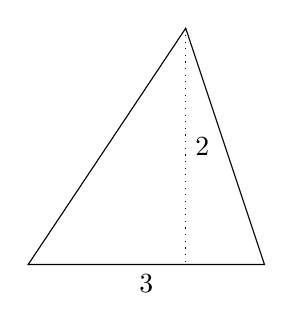
\begin{tikzpicture}
            \draw (0,0)--node[midway,below] {3} (3,0)--(2,3)--cycle;
            \draw [dotted] (2,3)--(2,0) node [midway, right] {2} ;
        \end{tikzpicture}
    \end{figure}
\end{minipage}
\hfill
\begin{minipage}[t]{0.30\textwidth}
    \exo{Calculer}{AireBasique9}\\
    \begin{figure}[H]
        \centering
        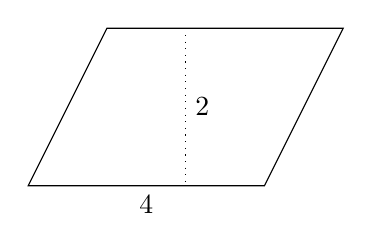
\begin{tikzpicture}
            \draw (0,0)--node [midway,below] {4} (3,0)-- (4,2)--(1,2)--cycle;
            \draw[dotted] (2,2)-- (2,0) node [midway,right] {2};
        \end{tikzpicture}
    \end{figure}
\end{minipage}

\begin{minipage}[t]{0.30\textwidth}
    \exo{Calculer}{AireBasique10}\\
    \begin{figure}[H]
        \centering
        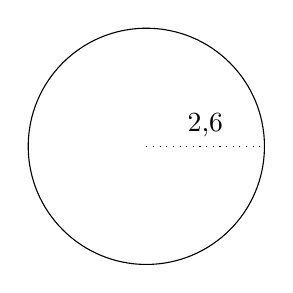
\begin{tikzpicture}
            \draw (0,0) circle (1.5);
            \draw[dotted] (0,0)--(1.5,0) node [midway, above] {2,6};
        \end{tikzpicture}
    \end{figure}
\end{minipage}
\hfill
\begin{minipage}[t]{0.30\textwidth}
    \exo{Calculer}{AireBasique11}\\
    \begin{figure}[H]
        \centering
        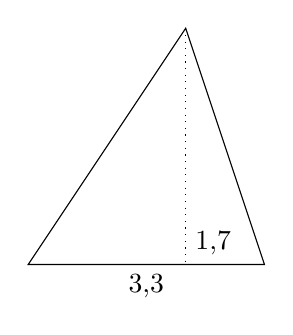
\begin{tikzpicture}
            \draw (0,0)--node[midway,below] {3,3} (3,0)--(2,3)--cycle;
            \draw [dotted] (2,3)--(2,0) node [above right] {1,7} ;
        \end{tikzpicture}
    \end{figure}
\end{minipage}
\hfill
\begin{minipage}[t]{0.30\textwidth}
    \exo{Calculer}{AireBasique12}\\
    \begin{figure}[H]
        \centering
        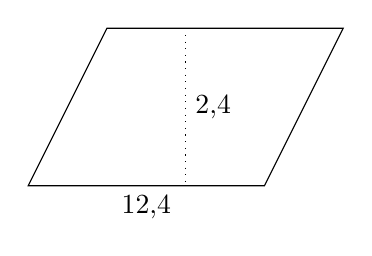
\begin{tikzpicture}
            \draw (0,0)--node [midway,below] {12,4} (3,0)-- (4,2)--(1,2)--cycle;
            \draw[dotted] (2,2)-- (2,0) node [midway,right] {2,4};
        \end{tikzpicture}
    \end{figure}
\end{minipage}